\section{INITIAL SHEAR MODULUS OF SOILS 土的初始剪切模量}

\Paragraph{Well-Shooting Method  地震测井试验}

\begin{paracol}{2}
    
    \citet{Miller1972545}  show that the geophysical exploration test comprises several types of practical methods (cross-hole, down-hole, up-hole, surface refraction and surface-vibration mothods).
    
    The down-hole method is to generate shear waves by hitting horizontally a wooden plate placed on the ground surface, so that velocity transducers clamped in a borehole receive such shear waves. To say more precisely, several velocity transducers are concurrently clamped in the borehole, which allow velocity measurement of a shear wave passing through a section ·between one transducer and the another.
    
    When the shear wave velocity $V_s$ is measured, shear modulus $G$ can be calculated by the following equation :

    \switchcolumn

    \citet{Miller1972545}表明,地球物理勘探试验包含几种类型的实用方法:横孔,井下,井上,表面折射和表面振动方法。
    
    井下方法是通过水平击打放置在地面上的木板来产生剪切波,以便夹在井眼中的速度传感器接收这些剪切波。 更准确地说,是将多个速度传感器同时夹紧在钻孔中,从而可以测量穿过一个传感器与另一个传感器之间的截面的剪切波的速度。
    
    当测量剪切波速度$V_s$时,剪切模量$G$可以通过以下公式计算:

\end{paracol}
    
\begin{align}
    G=\rho{}V_s^2(\rm{kg/cm^2})
    \label{equation:1}
\end{align}

\begin{paracol}{2}
    \noindent where $\rho$: mass density.

    This is the procedure called the well-shooting test by means of shear waves, on which \citet{Kitsunezaki19671,Shima19681301, Shima1969819, Imai197017} have already published their respective reseach papers.

    \switchcolumn

    \noindent 式中$\rho$:质量密度。

    这就是通过剪切波进行的所谓的地震测井试验程序,\citet{Kitsunezaki19671,Shima19681301, Shima1969819, Imai197017}已经在此上发表了各自的研究论文。

\end{paracol}

\Paragraph{Shear Strain Amplitude in Soil Deposits 土壤沉积物中的剪切应变幅值}

\begin{paracol}{2}
    
    Initial shear modulus can be defined as shear modulus at infinitely small shear strain amplitude.
    
    It is therefore necessary to obtain shear strain amplitude in soil deposits when the wellshooting test by means of shear waves is to be conducted.
    
    The reslt of the well-shooting test which was performed in a soft clay deposit, as an example, is shown in \autoref{figure:1}. The authors tried to calculate shear strain amplitude in a soft soil deposit from wave forms shown in \autoref{figure:1} with the following procedure: 

    \switchcolumn

    初始剪切模量可以定义为无限小剪切应变幅值下的剪切模量。
    
    因此,当要通过剪切波进行地震测井试验时,有必要获得土壤沉积物中的剪切应变振幅。
            
    例如,在软黏土矿床中进行的地震测井试验的结果如\cnfigureref{figure:1}所示。作者试图通过\cnfigureref{figure:1}所示的波形计算软土矿床中的剪切应变幅值,其中 步骤如下:

\end{paracol}


\begin{figure*}[!htb]
    \begin{minipage}[t]{0.66\textwidth}
        \centering
        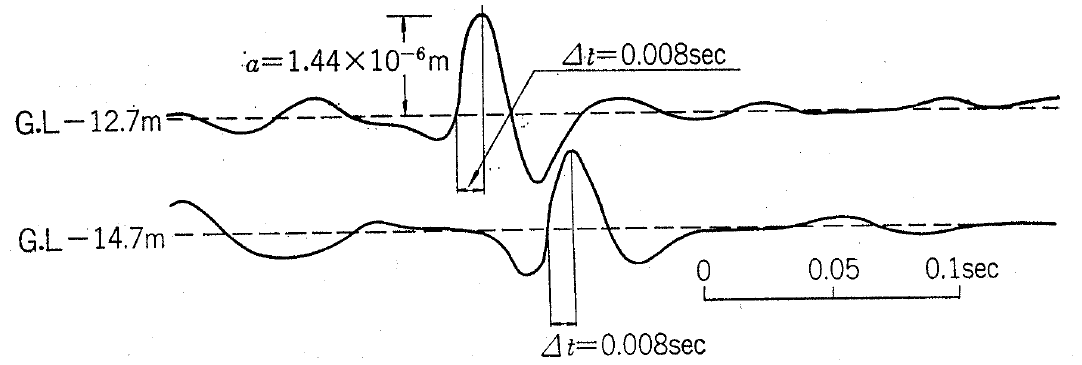
\includegraphics[width=\textwidth]{figures/figure-1.png}
        \caption{An example of shear wave velocity measurement}
        \addtocounter{figure}{-1}
        \vspace{-5pt}
        \renewcommand{\figurename}{图}
        \caption{剪切波速度测量示例}
        \renewcommand{\figurename}{Figure}
        \label{figure:1}
    \end{minipage}
    \begin{minipage}[t]{0.32\textwidth}
        \centering
        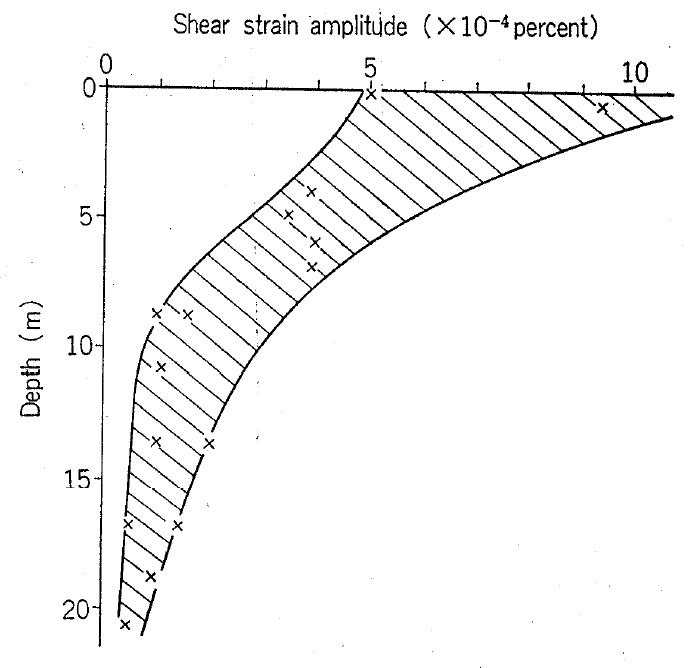
\includegraphics[width=\textwidth]{figures/figure-2.png}
        \caption{Estimated shear strain·amplitude at various depths}
        \addtocounter{figure}{-1}
        \vspace{-5pt}
        \renewcommand{\figurename}{图}
        \caption{各种深度的估计剪切应变振幅}
        \renewcommand{\figurename}{Figure}
        \label{figure:2}
    \end{minipage}
\end{figure*}


\begin{paracol}{2}
    
    (1) Calibration curves of the velocity transducers were firstly determined by shaking table in the laboratory.
    
    (2) On the assumption that principal shear wave should be represented by that of harmonic motion, the maximum shear d~splacement amplitude $\Delta{}x$ was estimated by the use of the calibration curves to be the following value:

    \switchcolumn
    
    (1)首先在实验室中通过振动台确定速度传感器的校准曲线。
            
    (2)假设应以谐波运动代表主剪切波,通过使用校准曲线将最大剪切位移振幅$\Delta{}x$估算为以下值:

\end{paracol}

\begin{align}
    \Delta{}x=0.0000144(\rm{m})
    \label{equation:2}
\end{align}

\begin{paracol}{2}    

    (3) On the other hand, thickness of soil deposit $\Delta{}H$ subject to shear displacement of $\Delta{}x$ can be calculated as follows :

    \switchcolumn
    
    (3)在 另一方面,受剪切位移$\Delta{}x$影响的土壤沉积物$\Delta{}H$的厚度可按以下公式计算:

\end{paracol}

\begin{align}
    \Delta{}H=V_s\cdot{}\Delta{}t=90\times{}0.008=0.72(\rm{m})
    \label{equation:3}
\end{align}

\begin{paracol}{2}

    (4) Shear strain amplitude $\gamma$ can thus be calculated as follows :

    \switchcolumn
    
    (4)因此,剪切应变幅值$\gamma$可按以下公式计算:

\end{paracol}

\begin{align}
    \gamma=\dfrac{1.44\times{}10^{-6}}{0.72}=2.0\times{}10^{-6}
    \label{equation:4}
\end{align}

\begin{paracol}{2}

    Shear strain amplitude obtained in the above procedure are plotted in \autoref{figure:2}, which shows that shear strain amplitude thus obtained by the well-shooting test can be assumed to be less than $10^{-3}\%$ percent.
    
    In addition, when shear strain amplitude is $10^{-3}\%$, shear stress as calculated below is so small that the shear modulus obtained by the well-shooting test can be regarded as initial shear modulus :

    \switchcolumn

    在上述过程中获得的剪切应变振幅绘制在\cnfigureref{figure:2}中,该曲线表明,可以将通过地震测井试验获得的剪切应变振幅假定为小于$10^{-3}\%$。
    
    另外,当剪切应变幅值为$10^{-3}\%$时,如下计算的剪切应力是如此之小,以至于通过地震测井试验获得的剪切模量可以视为初始剪切模量:

\end{paracol}

\begin{align}
    \tau=\gamma{}G=10^{-5}\times{}110=0.0011(\rm{kg/cm^2})
    \label{equation:5}
\end{align}

\Paragraph{Shear Strength of Soil 土的抗剪强度}

\begin{paracol}{2}
    
    The soil element shown in \autoref{figure:3} is deformed due to random vibrations propagating from bedrock to surface during an earthquake. In this case, the deformation excited most significantly is mainly attributable to the shear wave.

    \switchcolumn

    \cnfigureref{figure:3}所示的土壤单元由于地震期间从基岩传播到地面的随机振动而变形。 在这种情况下,最显着激发的变形主要归因于剪切波。      \switchcolumn*

    The initial stress condition of the soil element is the $K_0$-condition, which means that initial effective stresses in vertical and horizontal direction are a $\sigma_v'$ and $K_0\sigma_v'$ respectively.

    \switchcolumn
       
    土元素的初始应力条件为$K_0$条件,这意味着垂直方向和水平方向的初始有效应力为分别为$\sigma_v'$和$K_0\sigma_v'$。
    
    \switchcolumn*

    The shear modulus obtained from the well-shooting test is calculated from the velocity of the shear wave, which propagate through the soil elements vertically in the $K_0$-condition.

    \switchcolumn
       
    从地震测井试验获得的剪切模量是根据剪切波的速度计算的,剪切波的速度在$K_0$条件下垂直传播通过土体颗粒。

\end{paracol}

\begin{figure*}[!htb]
    \begin{minipage}[t]{0.54\textwidth}
        \centering
        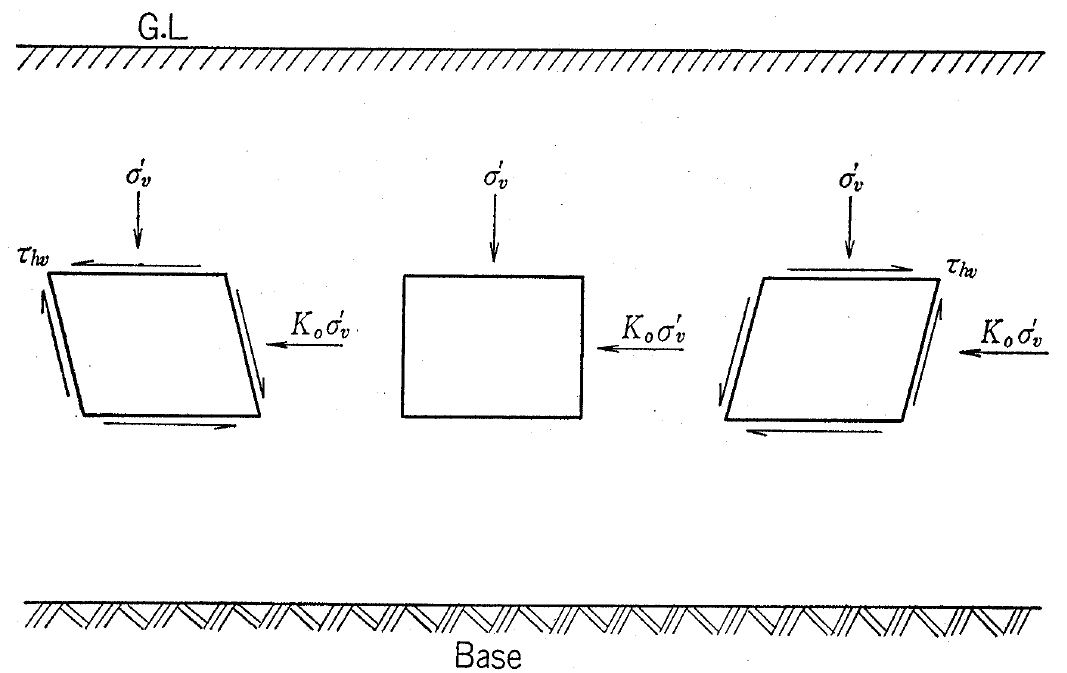
\includegraphics[width=\textwidth]{figures/figure-3.png}
        \caption{Conceptual field loading condition}
        \addtocounter{figure}{-1}
        \vspace{-5pt}
        \renewcommand{\figurename}{图}
        \caption{概念性的场地加载条件}
        \renewcommand{\figurename}{Figure}
        \label{figure:3}
    \end{minipage}
    \begin{minipage}[t]{0.42\textwidth}
        \centering
        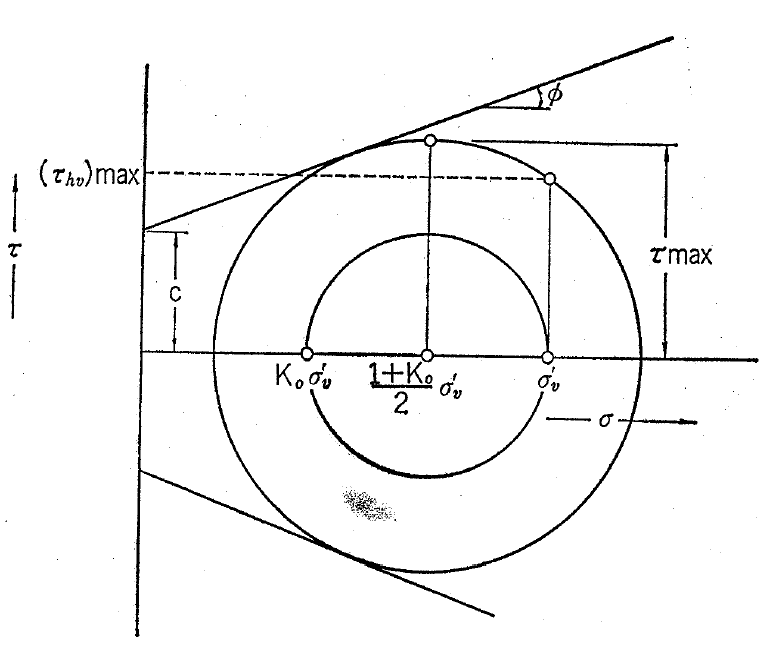
\includegraphics[width=\textwidth]{figures/figure-4.png}
        \caption{Mohr' s  circles and maximum shear stress}
        \addtocounter{figure}{-1}
        \vspace{-5pt}
        \renewcommand{\figurename}{图}
        \caption{莫尔圆和最大切应力}
        \renewcommand{\figurename}{Figure}
        \label{figure:4}
    \end{minipage}
\end{figure*}


\begin{paracol}{2}
    
    Therefore, it is reasonable that the shear strength of a soil deposit should be obtained by taking into account its initial stress condition. These problems have been sufficiently treated by Duncan, Seed and Hardin. According to these researches, when the soil element shown in \autoref{figure:3} comes to failure, the maximum lateral shear stress $(\tau_{hv})_{\rm{max}}$ is given on Mohr's circles as represented in \autoref{figure:4}. Taking the geometric relation in \autoref{figure:4} into consideration, the maximum lateral shear stress $(\tau_{hv})_{\rm{max}}$ will be

    \switchcolumn

    因此,合理的是应考虑其初始应力条件来获得土壤沉积物的剪切强度。\citet{Duncan1969101,Seed19711099,Hardin1973667}已经充分解决了这些问题。 根据这些研究,当\cnfigureref{figure:3}所示的土体单元破坏时,如\cnfigureref{figure:4}所示,在莫尔圆上给出最大横向剪应力$(\tau_{hv})_{\rm{max}}$。考虑到\cnfigureref{figure:4}中的几何关系,最大横向剪应力$(\tau_{hv})_{\rm{max}}$将是

\end{paracol}

\begin{align}
    S_u=(\tau_{hv})_{\rm{max}}=\left\{(\tau_{\rm{max}})^2-\left(\dfrac{1-K_0}{2}\sigma_v'\right)^2\right\}^{1/2}
    \label{equation:6}
\end{align}

\begin{paracol}{2}
    
    \newlength{\length}
    \settowidth{\length}{$K_0$: coefficient of earth pressure at rest}
    \noindent where \begin{minipage}[t]{\length}
        $K_0$: coefficient of earth pressure at rest, \\
        $\sigma_v'$: effective overburden pressure. 
    \end{minipage}\vspace{4pt}
    
    \switchcolumn

    \newlength{\cnlength}
    \settowidth{\cnlength}{$K_0$:静止时的土压力系数}
    \noindent 式中\begin{minipage}[t]{\cnlength}
        $K_0$:静止时的土压力系数,\\
        $\sigma_v'$:有效上覆土压力。
    \end{minipage}\vspace{4pt}

    \switchcolumn*

    In addition, if the cohesion $c$ and the angle of internal friction $\phi$ of soil are given, the maximum shear stress $\tau_{\rm{max}}$ can be·expressed by the following equation :

    \switchcolumn

    另外,如果给出了土的内聚力$c$和内摩擦角$\phi$,则最大剪切应力$\tau_{\rm{max}}$可以由下式表示:

\end{paracol}

\begin{align}
    \tau_{\rm{max}}=\dfrac{1+K_0}{2}\sigma_v'\sin\phi+c\cos\phi
    \label{equation:7}
\end{align}

\begin{paracol}{2}
    
    Substituting \autoref{equation:7} into \autoref{equation:6}, the shear strength $S_u$ of the soil element shown in \autoref{figure:4} can be given as follows :

    \switchcolumn

    将\cnequationref{equation:7}代入\cnequationref{equation:6},\cnfigureref{figure:4}所示的土体的抗剪强度$S_u$可以给出如下:

\end{paracol}

\begin{align}
    S_u=\left\{\left(\dfrac{1+K_0}{2}\sigma_v'\sin\phi+c\cos\phi\right)^2-\left(\dfrac{1-K_0}{2}\sigma_v'\right)^2\right\}^{1/2}
    \label{equation:8}
\end{align}

\begin{paracol}{2}
    
    However, the actual shear strength in soil deposit cannot be expressed so easily as above. For example, the process of development of the pore water pressure in the soil element vary with respective earthquakes, so that the effective overburden pressure and coefficient of earth pressure at rest are not constant, varying from the state of rest to the state of failure. The shear strength in a soil deposit cannot be exactly obtained for the above reason. Accordingly, it is realistic that the shear strength of a soil is calculated based on the assumption that the initial stress condition continues to the state of failure. The soil parameters in \autoref{equation:8} are determined by the following conditions : 

    \switchcolumn

    但是,土壤沉积物中的实际抗剪强度不能像上面那样容易地表达。 例如,土壤单元中孔隙水压力的发展过程随地震而变化,因此有效的上覆压力和静止时的土压力系数不是恒定的,从静止状态到破坏状态都不同。 由于上述原因,不能精确地获得土壤沉积物中的剪切强度。 因此,现实的是,基于初始应力条件持续到破坏状态的假设来计算土壤的剪切强度。\cnequationref{equation:8}中的土壤参数由以下条件确定:

    \switchcolumn*

    \begin{enumerate}
        \item The cohesion $c$ and the angle of internal friction $\phi$ are determined by the expression of total stress of the unconsolidated-undrained triaxial compression test.
        \item Brooker and Ireland have reported that the close relation were observed among the coefficient of earth pressure at rest $_K0$, the plasticity index $I_p$ and the overconsolidated ratio OCR as shown in \autoref{figure:5}. The value of $K_0$ to be required in \autoref{equation:8} was determined by the relation between Ip and OCR shown in \autoref{figure:5}.
    \end{enumerate}

    \switchcolumn

    \begin{enumerate}
        \item 内聚力$c$和内摩擦角$\phi$由不固结不排水三轴压缩试验的总应力表达式确定。
        \item \citet{Brooker19651}报告说,静止土压力系数$K0$,可塑性指数$I_p$和超固结比OCR之间存在密切关系,如\cnfigureref{figure:5}所示。\cnequationref{equation:8}中要求$K_0$的值由$I_p$与OCR之间的关系确定,如\cnfigureref{figure:5}所示。
    \end{enumerate}

\end{paracol}

\begin{figure*}[!htb]
    \begin{minipage}[t]{0.54\textwidth}
        \centering
        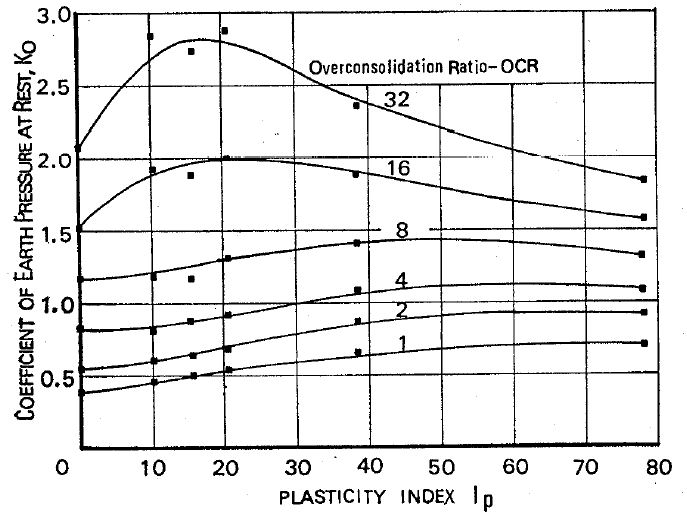
\includegraphics[width=0.9\textwidth]{figures/figure-5.png}
        \caption{Relationship between $K_0$, $I_p$ and OCR}
        \addtocounter{figure}{-1}
        \vspace{-5pt}
        \renewcommand{\figurename}{图}
        \caption{$K_0$,$I_p$和OCR之间的关系\citep{Brooker19651}}
        \renewcommand{\figurename}{Figure}
        \label{figure:5}
    \end{minipage}
    \begin{minipage}[t]{0.42\textwidth}
        \centering
        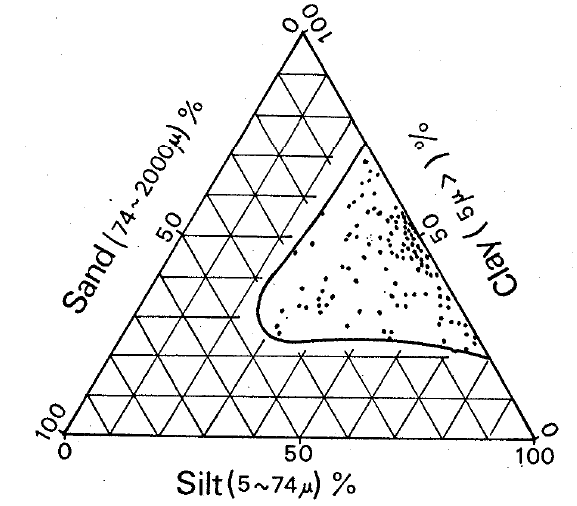
\includegraphics[width=\textwidth]{figures/figure-6.png}
        \caption{Trianguler classification chart}
        \addtocounter{figure}{-1}
        \vspace{-5pt}
        \renewcommand{\figurename}{图}
        \caption{三角分类图}
        \renewcommand{\figurename}{Figure}
        \label{figure:6}
    \end{minipage}
\end{figure*}


\Paragraph{Soil Classification 土体分类}

\begin{paracol}{2}
    
    The data on initial shear modulus, shear strength and N-value of the standard penetration test were obtained from 25 sites, which consisted of 15 alluvial deposits, 9 diluvial deposits, and 1 tertiary deposit.

    In order to describe the physical properties of soils used for this investigation, the triangular classification chart for the results of mechanical analysis is shown in \autoref{figure:6}, the results of plasticity and liquid limit test are shown in \autoref{figure:7} by the plasticity chart, while the relation between overconsolidation ratio and plasticity index are shown in \autoref{figure:8}, and the relation between degree of saturation and void ratio in \autoref{figure:9}.

    \switchcolumn

    标准贯入试验的初始剪切模量,剪切强度和N值的数据来自25个站点,包括15个冲积层,9个冲积层和1个三次层。
   
    为了描述用于该研究的土壤的物理性质,\cnfigureref{figure:6}所示为力学分析结果的三角分类图,塑性图则显示了可塑性和液体极限试验的结果,\cnfigureref{figure:7}所示。 固结率与塑性指标的关系如\cnfigureref{figure:8}所示,饱和度与空隙率的关系如\cnfigureref{figure:9}所示。

\end{paracol}

\begin{figure*}[!htb]
    \begin{minipage}[t]{0.32\textwidth}
        \centering
        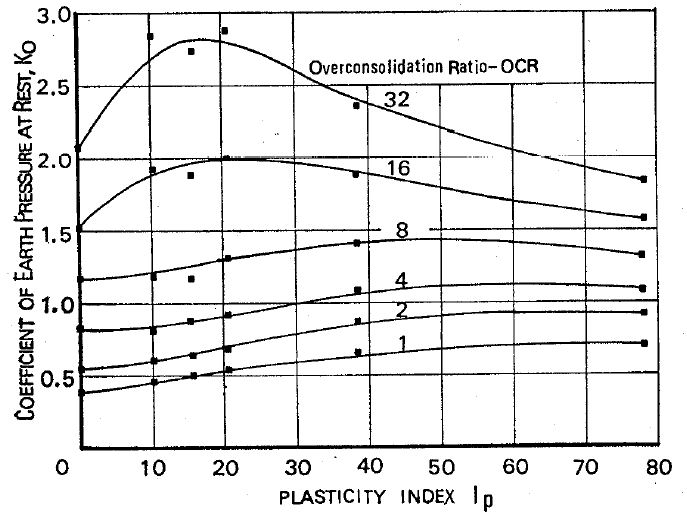
\includegraphics[width=\textwidth]{figures/figure-5.png}
        \caption{Relationship between $I_p$ and $W_L$}
        \addtocounter{figure}{-1}
        \vspace{-5pt}
        \renewcommand{\figurename}{图}
        \caption{$I_p$和$W_L$之间的关系\citep{Brooker19651}}
        \renewcommand{\figurename}{Figure}
        \label{figure:7}
    \end{minipage}
    \begin{minipage}[t]{0.32\textwidth}
        \centering
        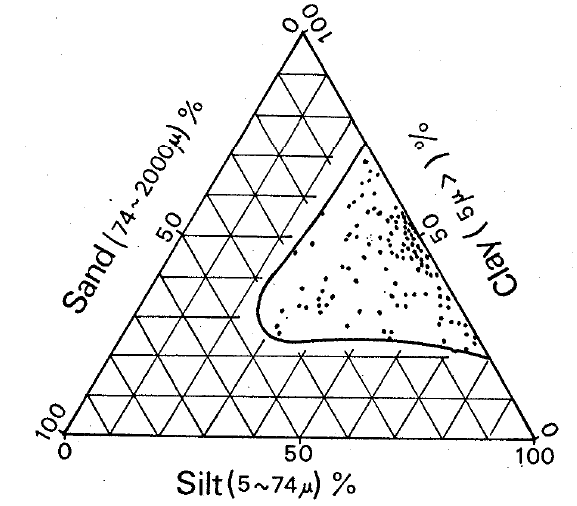
\includegraphics[width=\textwidth]{figures/figure-6.png}
        \caption{Relationship between OCR and $I_p$}
        \addtocounter{figure}{-1}
        \vspace{-5pt}
        \renewcommand{\figurename}{图}
        \caption{OCR和$I_p$之间的关系}
        \renewcommand{\figurename}{Figure}
        \label{figure:8}
    \end{minipage}
    \begin{minipage}[t]{0.32\textwidth}
        \centering
        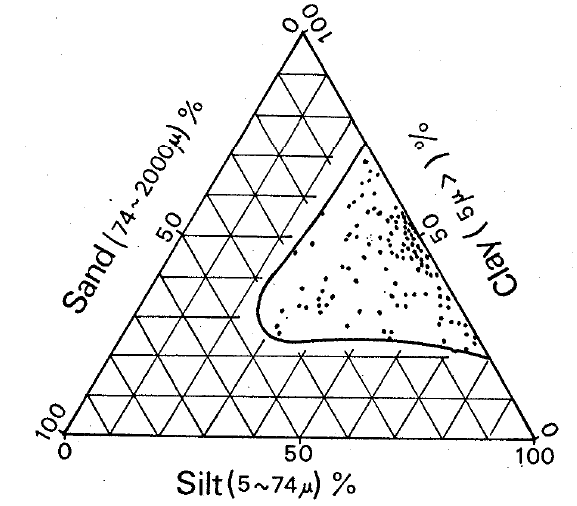
\includegraphics[width=\textwidth]{figures/figure-6.png}
        \caption{Relationship between $S_r$ and $e$}
        \addtocounter{figure}{-1}
        \vspace{-5pt}
        \renewcommand{\figurename}{图}
        \caption{$S_r$和$e$之间的关系}
        \renewcommand{\figurename}{Figure}
        \label{figure:9}
    \end{minipage}
\end{figure*}


\begin{paracol}{2}
    
    The physical properties of the soil used in this paper are summarized as follows from \autoref{figure:6}, \autoref{figure:7}, \autoref{figure:8} and \autoref{figure:9}: 

    \begin{enumerate}
        \item Soil belongs to the category of cohesive soil.
        \item The plasticity index has a wide range of distribution.
        \item The values of overconsolidation ratio range from 1.0 to 3.0.
        \item The values of void ratio range from 0.5 to 3.0, and most of the data are from 1.0 to 2.0.
        \item The values of the degree of saturation range from 90$\%$ to 100$\%$, and most of the data nearly 100$\%$.
    \end{enumerate}

    \switchcolumn

    \cnfigureref{figure:6},\cnfigureref{figure:7},\cnfigureref{figure:8}和\cnfigureref{figure:9}总结了本文使用的土壤的物理特性:
    \begin{enumerate}
        \item 土体属于黏性土。
        \item 可塑性指数分布范围广。
        \item 超固结比的值范围为1.0至3.0。
        \item 空隙率的值范围为0.5至3.0,大多数为1.0至2.0。
        \item 饱和度的值范围从90$\%$到100$\%$,大多数接近100$\%$。
    \end{enumerate}

\end{paracol}